\section{Development of the Bare-Metal Firmware}
\label{sec:firmware}
This Section describes the development of the bare-metal firmware.
First, we go over the firmware architecture, where we describe the technology stack and the architecture itself.
Second, we go over some components of the firmware that are either crucial to the firmware, or their implementation stands out in any way.

\subsection{Firmware Architecture}
\label{subsec:firmware-arch}
Firmware architecture can be described in many ways, we decided to show three ways in which we describe this firmware.
First, we describe the technology stack, describing what crates and libraries we built the hardware upon.
These libraries have mostly been described in the Section~\ref{sec:embedded_rust}.
The technology stack can be seen in the Figure~\ref{fig:firmware_tech_stack}.
When we go from the bottom, to the top, we can see that we access the hardware \acs{mcu} via two crates - the \textbf{stm32-rs} used to access peripheral circuits of the \acs{mcu} and the \textbf{cortex-m} crate used to access the \acs{arm} core of the \acs{mcu}.
The \textbf{stm32f4xx-hal} builds upon the \textbf{stm32-rs} crate and provides Hardware Abstraction Layer over the STM32F4 family and implements the \textbf{embedded-hal} traits.
The \textbf{cortex-m} crate is then used by the RTIC scheduler (described in the Section~\ref{subsec:mut_shared_state}).
As can be seen in the Figure, the firmware itself then builds upon all of these technologies - it accesses the HAL as some peripherals have their abstractions developed, for some special configurations the direct peripheral register access via \textbf{stm32-rs} is used, the RTIC scheduler is used for orchestrating the firmware and for some low-level assembly instructions the \textbf{cortex-m} crate for low level \acs{arm} core access is used.

\begin{figure}[H]
    \centering
    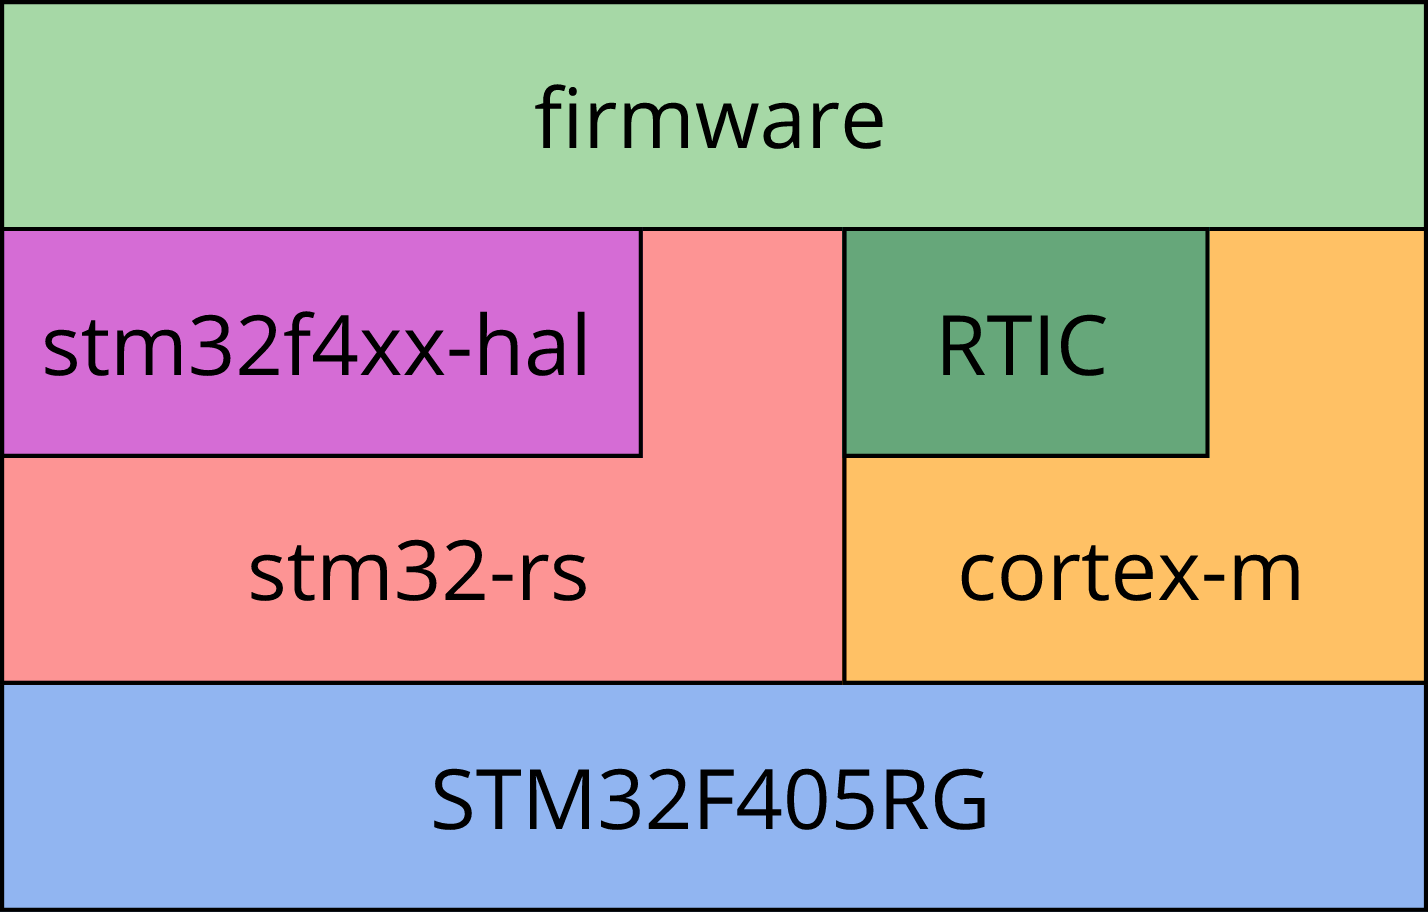
\includegraphics[width=0.5\textwidth]{obrazky/tech_stack}
    \caption{Bare-Metal firmware technology stack.}
    \label{fig:firmware_tech_stack}
\end{figure}

While the technology stack gives us vital information about the architecture, the architecture itself is much more complex and in theory could and should be independent on the used technologies\cite{thomas_pragmatic_2019}.
The architecture overview diagram can be seen in the Figure~\ref{fig:firmware_arch}.
The central part of the architecture is the Object Dictionary (described in Section~\ref{subsec:object_dictionary} and~\ref{subsec:object_dict_impl} (implementation-wise)).
The object dictionary contains the state of the stepper motor controller alongside with configuration.
Part of the object dictionary is also a persistent storage where its values are retained between reboots.
In the center of the firmware, there is also general state that stores variables outside the scope of the Object Dictionary and software failsafe mechanisms, that can manipulate bot the state and object dictionary.
When we look lower in the diagram, we can see that there are the communication interfaces that receive data from and send them to the outer world, usually to some high-level system.
On the other hand, when we look higher in the diagram, that's where the motion control systems operate, they get their data from the object dictionary (control values) and encoders and use these data for controlling the stepper motor driver \acs{ic}s.
The encoders and motor drivers are again connected to the outer world - meaning that they interact with it via the connected motors.

\begin{figure}[H]
    \centering
    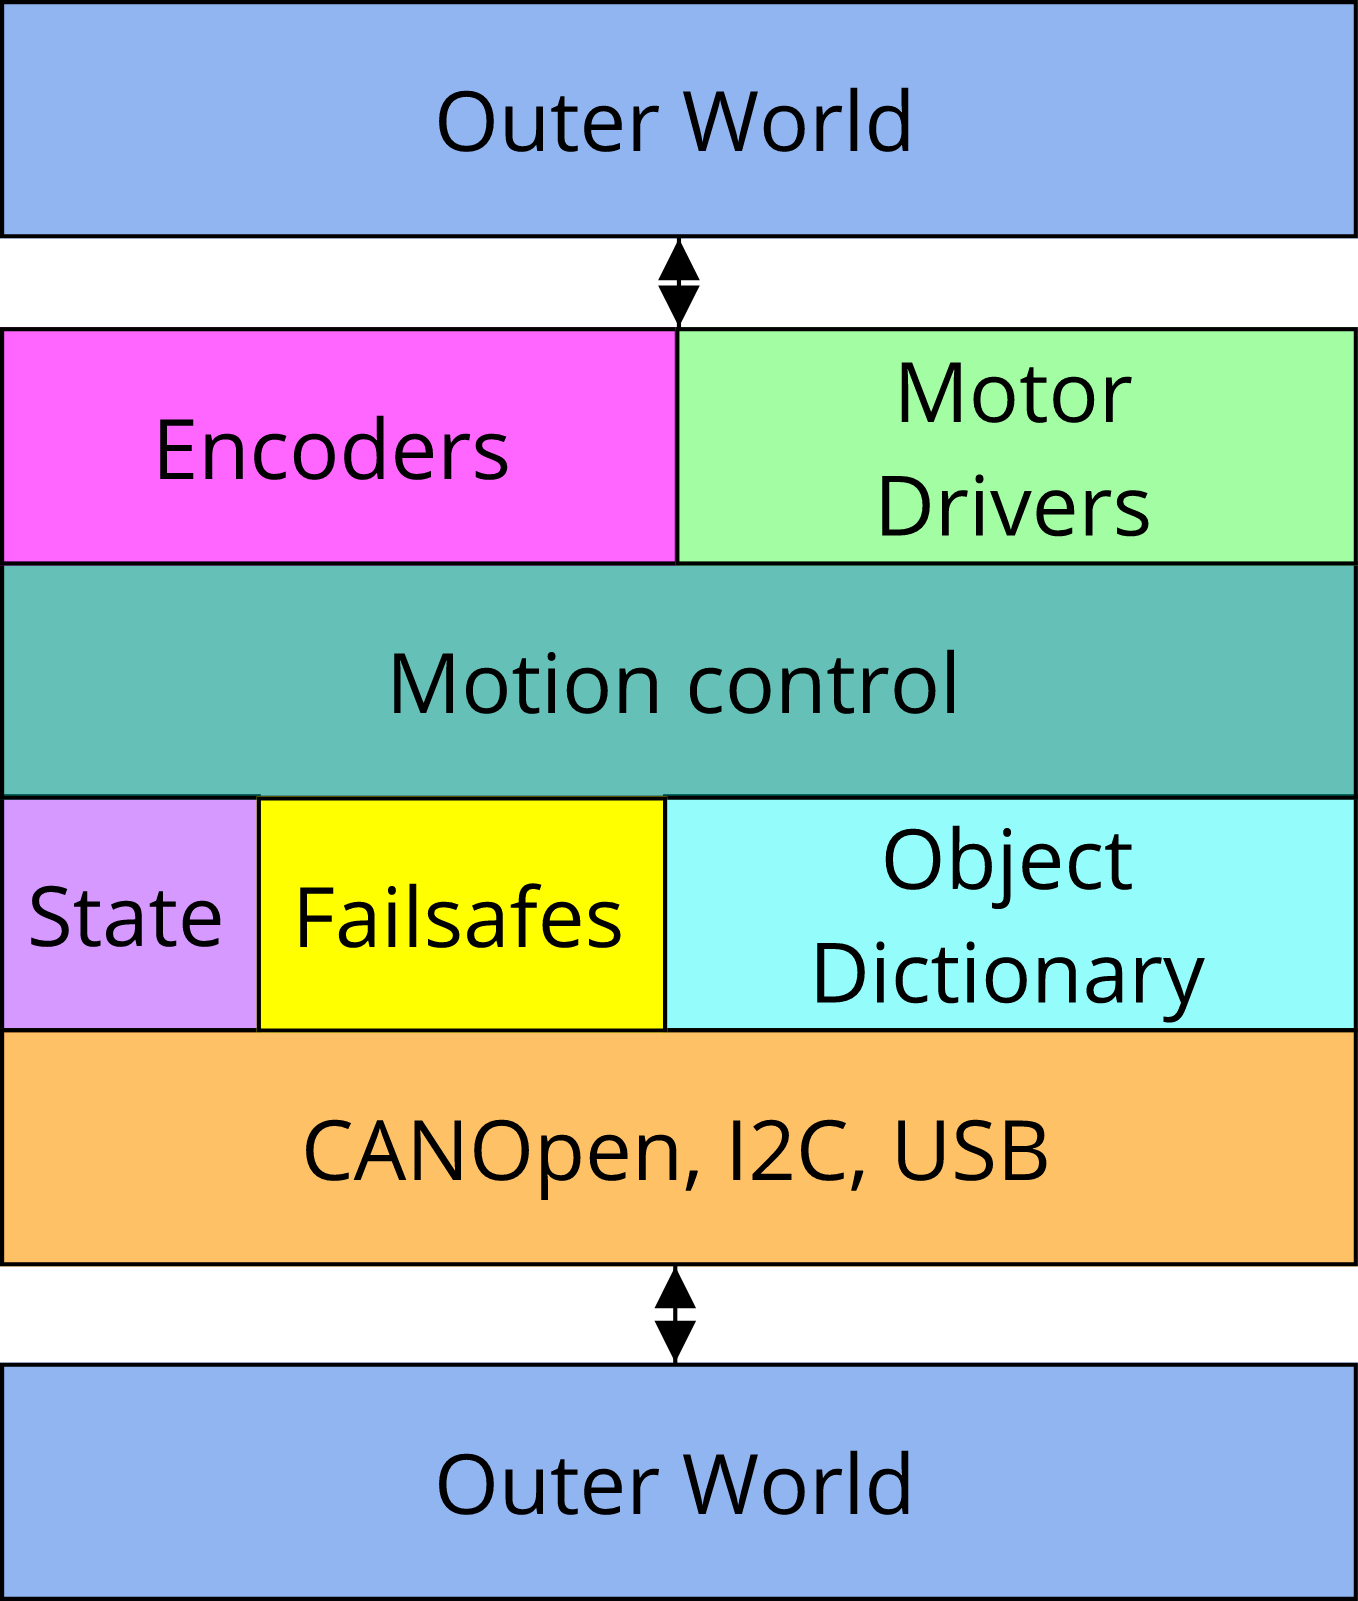
\includegraphics[width=0.5\textwidth]{obrazky/firmware_arch}
    \caption{Bare-Metal firmware architecture.}
    \label{fig:firmware_arch}
\end{figure}

There is one more final point of view on the architecture, which is connected with the project structure.
Given there are two projects - the bare-metal firmware, and the further-described control application, there is a need to share code between those two projects, e.g. share communication models.
An important distinction being, that the bare-metal firmware is also cross-compiled and cross-compiled in a \textbf{no\_std} environment.
Code sharing was solved by creating another project, that is \textbf{no\_std} and is simply called \textbf{shared}, both of the application projects statically link against it.
This can be seen in a diagram presented in the Figure~\ref{fig:component_arch}.
The project structure was adopted from\cite{aparicio_testing_nodate}, which proposes a project structure, that promotes code sharing and testability of all components.

\begin{figure}[H]
    \centering
    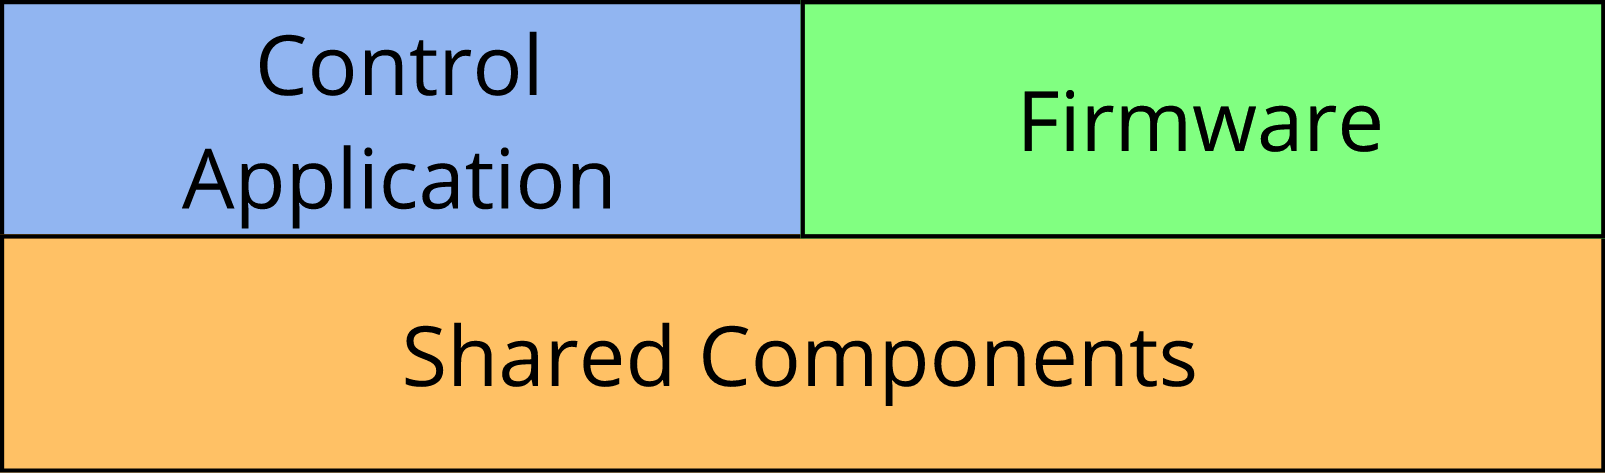
\includegraphics[width=0.5\textwidth]{obrazky/components}
    \caption{Component sharing between the bare-metal firmware and the Control Application.}
    \label{fig:component_arch}
\end{figure}

\subsection{Object Dictionary}
\label{subsec:object_dict_impl}
The importance and role of the Object Dictionary was described in the Sections~\ref{subsec:object_dictionary} and~\ref{subsec:firmware-arch}.
When designing the Object Dictionary, we wanted to design it so that it could be universally used and implemented in multiple ways (e.g. with persistent storage or without one).
The abstraction was done using traits.
The most important trait is the ObjectDictionary trait displayed in the Listing~\ref{lst:od_trait}.
This trait describes the Object Dictionary as a type, that contains information about battery voltage, temperature and an arbitrary number of axes.
The axis is also represented as a trait with accessor methods for specific axis settings (controller settings, current settings, etc.).

\begin{lstlisting}[caption={Trait for abstracting away the Object Dictionary.},label=lst:od_trait]
/// Trait for Object Dictionary abstraction
pub trait ObjectDictionary<const RESOLUTION: u32> {
    /// Returns battery voltage stored in the Object Dictionary.
    fn battery_voltage(&self) -> f32;
    /// Returns temperature stored in the Object Dictionary.
    fn temperature(&self) -> f32;
    /// Sets the battery voltage value in the Object Dictionary.
    fn set_battery_voltage(&mut self, battery_voltage: f32);
    /// Sets the temperature value in the Object Dictionary.
    fn set_temperature(&mut self, temperature: f32);
    /// Returns the configuration of a specific axis.
    fn axis(&self, axis: Axis) -> &dyn AxisDictionary<RESOLUTION>;
    /// Returns a mutable reference the configuration of a specific axis.
    /// This is the only way an axis configuration can be changed
    fn axis_mut(&mut self, axis: Axis) -> &mut dyn AxisDictionary<RESOLUTION>;
}
\end{lstlisting}

To implement a simple Object Dictionary, implementing these traits would be enough, but since we wanted to create an Object Dictionary whose values can be saved in an arbitrary storage, we needed to create another abstraction for storage.
Such an abstraction can be found in the Listing~\ref{lst:storage_trait}.
As can be seen in the Listing, the trait defines loading and saving values of 32-bit floats and boolean values for an arbitrary type of key, that implements the ObjectDictionaryKey.

\begin{lstlisting}[caption={Trait for abstracting away the Object Dictionary storage.},label=lst:storage_trait]
pub trait ObjectDictionaryStorage {
    fn save_f32<KEY: ObjectDictionaryKey>(&mut self,
        key: KEY, value: f32);
    fn save_bool<KEY: ObjectDictionaryKey>(&mut self,
        key: KEY, value: bool);
    fn load_f32<KEY: ObjectDictionaryKey>(&self,
        key: KEY) -> Option<f32>;
    fn load_bool<KEY: ObjectDictionaryKey>(&self,
        key: KEY) -> Option<bool>;
}
\end{lstlisting}

Using all the aforementioned traits we then developed Object Dictionary implementation called the PersistentStoreObjectDictionary, which is generic over the ObjectDictionaryStorage, meaning, that an arbitrary storage type can be used with it.
Similar to the Object Dictionary traits, we also needed to develop a Persistent Store Object Dictionary for axis data, which is also generic over the Object Dictionary Storage and can be seen in the Listing~\ref{lst:persistent_store_dict}.

\begin{lstlisting}[caption={Object Dictionary for persistently storing axis data.},label=lst:persistent_store_dict]
#[derive(Copy, Clone)]
pub struct PersistentStoreAxisDictionary<
    STORAGE: 'static + ObjectDictionaryStorage,
    const RESOLUTION: u32,
> {
    axis: Axis,
    mode: AxisMode,
    enabled: bool,
    target_velocity: Velocity,
    actual_velocity: Velocity,
    target_position: Position<RESOLUTION>,
    actual_position: Position<RESOLUTION>,
    current: CurrentSettings,
    velocity_controller_settings: ControllerSettings,
    position_controller_settings: ControllerSettings,
    velocity_feedback_control_enabled: bool,
    acceleration: f32,
    storage: &'static Mutex<RefCell<STORAGE>>,
}
impl<STORAGE: 'static + ObjectDictionaryStorage, const RESOLUTION: u32>
    AxisDictionary<{ RESOLUTION }> for PersistentStoreAxisDictionary<STORAGE, RESOLUTION>
{
    fn set_accelerating_current(&mut self, current: f32) {
        self.current.set_accelerating_current(current);
        self.storage.lock().borrow_mut().save_f32(
            Key::key_for_axis(AxisKey::AcceleratingCurrent, self.axis),
            current,
        );
    }
...
}
\end{lstlisting}

An important note is that now when any part of the code needs to access the Object Dictionary, it is done by hiding the real implementation behind dynamic dispatch based on the ObjectDictionary trait.

Since we are expecting that the only way a value can be written into the Object Dictionary is using the accessor methods, we employ buffering to make storage reads more scarce, therefore more making the ObjectDictionary more effective.
This basically means that at the firmware startup, all the values are loaded to \acs{ram} and the storage is not accessed when reading.

\subsection{Persistent storage using EEPROM emulation}
\label{subsec:eeprom}
In the previous Section, we discussed development of storage agnostic persistent Object Dictionary and in this section, the way we actually implemented the persistent storage is described.
Persistent storage on MCUs is generally solved by using non-volatile memory that can be either part of the MCU or an external component.
Different memory technologies may be used for both types of the storage.
In general, \acs{fram} (\acl{fram}), \acs{eeprom} (\acl{eeprom}), or flash memories are used.

In order to save space on the \acs{pcb}, save cost, and better utilize the MCU resources we decided to use the internal flash memory to store the user data apart from the driver firmware.
Even though the flash memory may seem straightforward to use since they are ubiquitous, their low level use is not that simple.
A flash memory is generally divided into sectors, that can be several kilobytes or megabytes large.
These sectors can be electrically erased - which means that every bit in the sector is set to 1.
Depending on the memory a word of a specific size can be programmed, but it is only possible to flip the bits in the word to zero~\cite{mansanet_ecorax_nodate, mansanet_ecorax_nodate-1}.
That means that to write a higher number to the word of the memory, the flash needs to be first erased and then programmed.
This is problematic for two reasons:
\begin{enumerate}
    \item sectors generally have the size of several kilobytes, meaning that when you'd want to update the value in the desired word, the whole sector would have to be read to some other memory, erased and then programmed again with the new, updated value,
    \item there is a limited number of whole sector erases, caused by the limitation of hardware.
\end{enumerate}

Fortunately, this problem can be solved by emulating the EEPROM memory as described in ST Application Note AN3969~\cite{stmicro_an3969_2011}.
The application note leverages two FLASH sectors of the same size, where one of them is marked as the active one and the second one is used when the first sector is full.
The working principle is described in the following paragraphs and can be seen in the Figure~\ref{fig:eeprom_emul}.

In the beginning, both of the sectors are erased and one of them is marked as active.
Data are then written to the first sector into simulated cells.
The cells contain a header (which can be understood as a key or a virtual address) and the data.
When a new write is requested, the data are appended behind the already stored data.
When a data with is read using the virtual address, or a key, the sector is traversed from its end, searching for the first occurrence of the key or address.
The first occurrence is the most recent value of the cell marked by the key.
This way we are able to store the value with a specific identifier (key, virtual address) in the flash multiple times.

When no more cells can be written to the active sector, the second sector is marked active, and the data are transmitted to the second sector, taking only the latest value of an identifier into account.
After the transfer, the first sector is erased.

\begin{figure}[H]
    \centering
    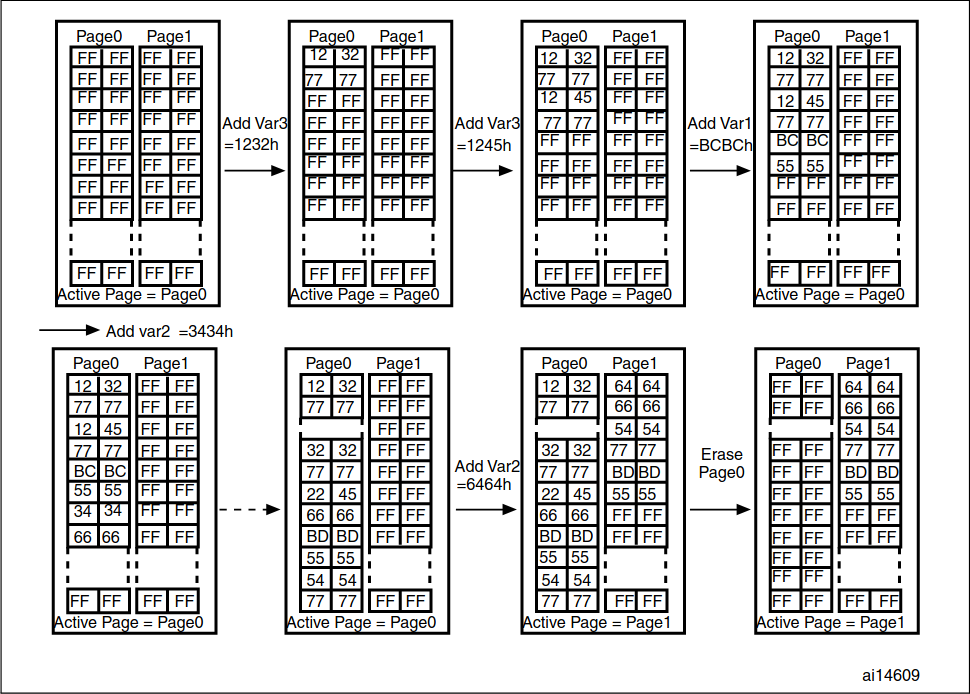
\includegraphics[width=\textwidth]{obrazky/eeprom_emul_principle}
    \caption{EEPROM emulation working principle~\cite{stmicro_an3969_2011}.}
    \label{fig:eeprom_emul}
\end{figure}

Even though the working principle of the EEPROM emulation is simple, there are some technical obstacles in the implementation.
The first obstacle is that the flash memory on the STM32 MCU is split into differently sized sectors, and it is required that the sectors have the same size.
Referring to the Reference Manual~\cite{stmicro_stm32f405rg_nodate} there are a some 16~kilobyte sectors that could be used for the emulation, as can be seen in the Figure~\ref{fig:flash_layout}.
Using the 128~kilobyte sectors would also be possible, but given their size copying values from one sector to another would take too much time and also read access times would be higher.

\begin{figure}[H]
    \centering
    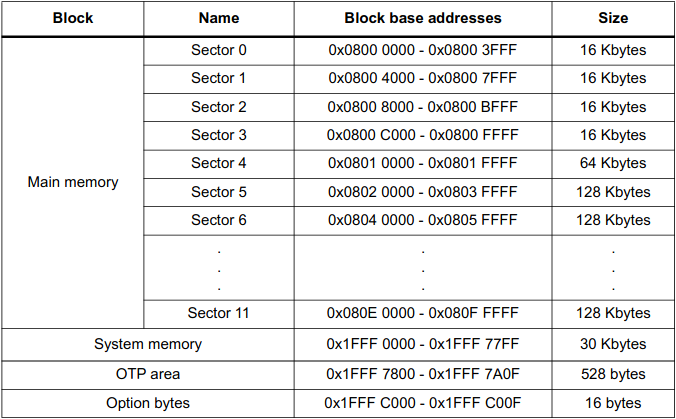
\includegraphics[width=0.8\textwidth]{obrazky/flash_stm}
    \caption{EEPROM emulation working principle~\cite{stmicro_stm32f405rg_nodate}.}
    \label{fig:flash_layout}
\end{figure}

There is however a problem with using the sectors in the beginning of the flash memory as that is where the firmware is usually stored.
The solution to this problem is by leaving the first sector (Sector 0) for the vector table and instructing the linker to place the \textbf{.text} section of the program further in the memory.
According to the documentation of the \textbf{cortex-m} Rust crate~\cite{rust_embedded_devices_wg_rust-embeddedcortex-m_2021}, this can be achieved by adding the line \textbf{\_stext = ORIGIN(FLASH) + OFFSET} to the linker script, where the \textbf{OFFSET} shall be replaced with the offset of the target sector where we want our program to be stored, in our case \textbf{0x0000C000}, which indicates the start of the Sector 3.

As for the actual implementation of the emulation for the STM32F405, we decided to develop our own, as no suitable Rust crate was available for it.
The development was inspired by a crate that implemented the emulation for STM32F103~\cite{dubrov_idubroveeprom_2020} and by following the implementation in the Application Note.
The functions from flash memory access were adopted from an as of the time of writing unmerged Pull Request into the STM32F4 HAL~\cite{astro_implement_2020}.
An example of accessing the emulated persistent storage can be seen in the following Listing~\ref{lst:eeprom}.

\begin{lstlisting}[caption={An example use of the emulated persistent storage.},label=lst:eeprom]
let mut store = Storage::new(device.FLASH);
store
    .init()
    .expect("Failed to initialize emulated storage.");
store.write_f32(0xbeef, 3.14);
let read = store.read_f32(0xbeef).unwrap();
assert_eq!(read, 3.14);
\end{lstlisting}

As can be seen in the Listing~\ref{lst:eeprom}, first we create the object with a parameter of the flash peripheral, then we initialize the emulated storage - this prepares the sectors that are supposed to be used and then we perform a simple write and read operations on the storage.

\subsection{CANOpen Implementation}
\label{subsec:canopen_impl}
The CAN bus on STM32 is implemented in hardware in the bxCAN peripheral.
This peripheral is the same for all of the STM32F \acs{mcu}s, only with slight differences in filter banks and message mailbox sizes.
Given this fact it was possible to develop a crate that supports all of the STM32 \acs{mcu}s, the crate is called \textbf{bxcan} and is developed the stm32-rs organization.

In the past projects described in Chapter~\ref{ch:related_work}, we utilized our own implementation of a driver for the bxCAN peripheral, but since the \textbf{bxcan} crate is well maintained, documented and tested, we decided to discontinue development of the driver and migrate to \acs{bxcan}.

In order to implement the CANOpen protocols described in the Section~\ref{subsec:canopen}, we developed a simple wrapper over the \textbf{bxcan} crate.
The wrapper is basically a simple proxy that transforms CANOpen protocol data to CAN frames and sends them and parses received CAN frames into CANOpen protocol data.
Upon initialization, the wrapper first configures the bxCAN peripheral, enables interrupts and enables the peripheral itself.

The bxCAN initialization in the wrapper can be seen in the Listing~\ref{lst:canopen_wrapper}.
\begin{lstlisting}[caption={Initializing the bxCAN peripheral in the CANOpen wrapper.},label=lst:canopen_wrapper]
let mut bus = Can::new(bus);
bus.configure(|config| {
    config.set_bit_timing(0x001a000b);
});
bus.enable_interrupts(
    Interrupts::FIFO0_MESSAGE_PENDING | Interrupts::FIFO1_MESSAGE_PENDING,
);
bus.modify_filters()
    .clear()
    .enable_bank(0, Mask32::accept_all());
bus.set_automatic_wakeup(true);
nb::block!(bus.enable()).unwrap();
\end{lstlisting}

When an interrupt handler is invoked, the function \textbf{process_incoming_frame} is called and it returns the type of the CANOpen protocol message, alongside with the received frame.
If the frame contains valid CANOpen message, the CAN frame is further parsed, for example to decode the contents of the PDO as can be seen in the Listing~\ref{lst:can_parse}

\begin{lstlisting}[caption={Initializing the bxCAN peripheral in the CANOpen wrapper.},label=lst:can_parse]
pub fn rx_pdo2<OD, const R: u32>(frame: &Frame, state: &mut DriverState<OD, R>)
where
    OD: ObjectDictionary<R>,
{
    if frame.data().is_none() {
        defmt::warn!("Invalid RxPDO2 received.");
        return;
    }
    if let Ok(pdo) = RxPDO2::try_from(frame.data().unwrap().as_ref()) {
        state
            .object_dictionary()
            .axis_mut(Axis::Axis1)
            .set_target_velocity(Velocity::new(pdo.axis1_velocity));
        state
            .object_dictionary()
            .axis_mut(Axis::Axis2)
            .set_target_velocity(Velocity::new(pdo.axis2_velocity));

        state.invalidate_last_received_speed_command_counter();
    } else {
        defmt::warn!("Malformed RxPDO2 received.");
    }
}
\end{lstlisting}
In the Listing, we can also see accessing the generic ObjectDictionary via the structure \textbf{DriverState}.

\subsection{I2C Implementation}
\label{subsec:i2c_impl}

\subsection{USB}
\label{subsec:usb_impl}

\subsection{Stepper control}
\label{subsec:stepper_control}
Movement of stepper motors, controlled using the stepper motor driver \acs{ic}s is generally controlled using the \textbf{STEP/DIR} interface.
This interface consists of two signals, the first of them named~\textbf{STEP} is a square wave signal with variable frequency, where the edges (rising, falling, or both) instruct the driver to move the motor by a microstep.
On the other hand, the second signal named \textbf{DIR} is generally a logic signal, whose logic level denotes the direction of the shaft movement.

Apart from these two digital signals, there is usually an analog signal that is used to set the motor phase current.
In more modern stepper drivers, this analog signal is replaced by a serial digital interface, allowing for finer current setting.

The \textbf{STEP} signal can be generated either in software (by changing the output logical level of a \acs{gpio} pin) or in hardware by utilizing a \acs{pwm} signal with duty cycle of 50 \%.
Both of these approaches have their limitations and advantages.
Generating the signal in software has the advantage of being able to easily count the number of microsteps the motor was commanded to do, on the other hand the upper limit of the maximal frequency is much lower than with hardware generation and this technique uses more computational resources as the signal is generally generated using an interrupt on timer overflow, where the signal logic level needs to be toggled (which requires branching) and the pulse counter needs to be accessed.
Using a timer with \acs{pwm} allows for much higher maximal frequencies, on the other hand counting the pulses can prove to be quite hard.
This issue will be described in more detail in the Section~\ref{subsec:simulated_encoders}.

We decided to utilize the \textbf{STEP} signal generation done by the hardware as we wanted to offload the work from the \acs{mcu} core.

To abstract the real implementation we created a trait (see Section~\ref{subsec:traits}) for setting the microstepping frequency, as can be seen in the Listing~\ref{lst:step_gen_trait}.
Using this trait the software controlling the stepper driver \acs{ic} can use either hardware or software \textbf{STEP} signal generator.

\begin{lstlisting}[caption={Trait for abstracting STEP generation.},label=lst:step_gen_trait]
/// This trait is an abstraction over hardware/software that is capable of generating square wave signal of specific frequency.
/// It is generally implemented by timers.
pub trait StepGenerator {
    /// Sets output frequency of the generator.
    ///
    /// # Arguments
    /// * `frequency` - frequency of the output square wave signal
    fn set_step_frequency(&mut self, frequency: Hertz);
}
\end{lstlisting}

In our case, the trait is implemented by the abstractions over the \acs{mcu}'s advanced control timers 1 and 8.
The abstractions over the timers are based on the timer implementations that can be found in the \textbf{stm32f4xx-hal}, but are preconfigured to generate output \acs{pwm} signals and also to act as a master timer generating clock signal for other timer on compare.

Using this trait, we were able to define a struct which describes the TMC2100 driver as can be seen in the Listing~\ref{lst:tmc2100}.

\begin{lstlisting}[caption={TMC2100 driver.},label=lst:tmc2100]
pub struct TMC2100<G, STEP, DIR, DAC> {
    generator: G,
    _step_pin: STEP,
    dir_pin: DIR,
    current_dac: DAC,
    sense_r: f32,
    microsteps_per_revolution: f32,
}
\end{lstlisting}
In the Listing, we can see, that the driver contains a generic generator, has ownership of the \textbf{STEP} pin (so that no other peripheral can access it), has ownership of the \acs{DIR} pin, \acs{dac} current reference and knows the value of the sense resistor for current setting and microsteps per revolution for \textbf{STEP} output frequency setting.

For a more seamless integration with the motion controller described in the Section~\ref{subsec:motion_control} the trait \textbf{StepperDriver} was declared as can be seen in the Listing~\ref{lst:stepper_driver_trait}.

\begin{lstlisting}[caption={Trait for abstracting the stepper motor driver IC.},label=lst:stepper_driver_trait]
/// This trait is an abstraction over stepper drivers.
/// Generally the drivers have two functions - generate steps and set output current.
pub trait StepperDriver {
    /// Sets output frequency of the driver.
    /// this shall be the angular frequency of the output shaft in revolutions per second.
    ///
    /// # Arguments
    /// * `frequency` - frequency of the output motor shaft in revolutions per second
    fn set_output_frequency(&mut self, frequency: f32);

    /// Sets the target current the driver shall drive the stepper motor with.
    ///
    /// # Arguments
    /// * `current` - the desired current in Amps
    fn set_current(&mut self, current: f32);
}
\end{lstlisting}

This trait was then implemented for the TMC2100 structure, implementing the stepper control itself, as is shown in the Listing~\ref{lst:stepper_driver_impl}.

\begin{lstlisting}[caption={Implementing the StepperDriver trait for TMC2100.},label=lst:stepper_driver_impl]
impl<G, STEP, DIR, DAC> StepperDriver for TMC2100<G, STEP, DIR, DAC>
where
    G: StepGenerator,
    DIR: embedded_hal::digital::v2::OutputPin,
    DAC: DACChannel,
{
    fn set_output_frequency(&mut self, frequency: f32) {
        if frequency < 0.0 {
            self.dir_pin.set_high().ok();
        } else {
            self.dir_pin.set_low().ok();
        };
        self.generator.set_step_frequency(Hertz::new(
            (frequency.abs() * self.microsteps_per_revolution) as u32,
        ))
    }
    fn set_current(&mut self, current: f32) {
        let voltage = (current.abs() * MAX_V_REF as f32 / V_FS * (self.sense_r + R_OFFSET) / 0.707) as u16;
        self.current_dac.set_output_voltage(voltage.min(MAX_V_REF));
    }
}
\end{lstlisting}

\subsection{Simulated encoders}
\label{subsec:simulated_encoders}
The SM4 stepper motor controller is meant to be used without hardware encoder in its default hardware configuration.
This requirement was caused by the reasoning that the motor controller is also targeted for the BPC-PRP course, where students use the distance driven by the wheels to calculate the robot's position in the world's reference frame.
Thankfully, with stepper motor, it is quite easy to simulate encoders by counting the number of microsteps the motor was supposed to move by.
The simulated encoders do not provide real feedback from the system, on the other hand when some conditions are met (no step skipping - no motor overloading), the measurement from them can be quite reliable.

As we already discussed in the Section~\ref{subsec:stepper_control}, we decided to not use counting the microsteps in software, but in hardware instead.
This is done by chaining timers in the \acs{mcu}.
We already mentioned that the timers used to generate \textbf{STEP} signal are configured to be the clock source for other timers, and by counting the clock cycles, we are able to count the number of microsteps the motor was commanded to turn by.

The working principle is really simple and also saves computational power of the \acs{mcu}, but has one disadvantage - the amount of microsteps per sampling period is too low to be used for velocity control, as the difference between the consecutive position reads is usually zero and only sometimes 1.
This poses a big problem for motor control systems of any kind.

Let's have a look at the implementation.
Similarly to what we did with the \textbf{STEP} signal generators, we also declared a trait to abstract away the thing that counts the pulses, so that on the outside it doesn't matter how the counting works.
The trait can be seen in the Listing~\ref{lst:step_counter}.

\begin{lstlisting}[caption={Counter trait for counting STEP pulses.},label=lst:step_counter]
/// Trait used to abstract STEP pulse and other counters.
pub trait Counter {
    /// Return the current internal value of the counter.
    fn get_value(&self) -> u32;
    /// Resets the internal value of the counter.
    fn reset_value(&mut self);
}
\end{lstlisting}
The trait was implemented for the timers 2 and 5 of the \acs{mcu}.

Apart from this trait, an abstraction over the whole encoded was developed.
The abstraction utilizes const generics to define encoder resolution and can be seen in the Listing~\ref{lst:encoder_trait}.

\begin{lstlisting}[caption={Encoder trait for abstracting encoders.},label=lst:encoder_trait]
/// A trait abstracting common encoder functionality.
/// It is suitable for both incremental and absolute encoders.
/// It is designed so its [`Self::sample()`] shall be periodically called with known fixed period,
/// which allows for velocity calculations.
pub trait Encoder<const RESOLUTION: u32> {
    /// Returns the velocity measured by the encoder.
    /// This value is generally calculated from consecutive position readings.
    fn get_velocity(&self) -> Velocity;

    /// Returns the current position of the shaft.
    fn get_position(&self) -> Position<RESOLUTION>;

    /// Sets the sampled position to zero.
    /// This is applicable only with incremental encoders.
    /// Absolute encoders might offset the zero by software.
    fn reset_position(&mut self) -> Position<RESOLUTION>;

    /// This functions shall be periodically called to sample the encoder.
    /// Sampled values are used for position and velocity readings.
    fn sample(&mut self);

    /// This method shall be called with non-directional encoders whenever there is a change of rotation direction.
    /// # Arguments
    /// * `direction` - indicates whether the shaft is now turning in the clockwise or counterclockwise direction.
    fn notify_direction_changed(&mut self, direction: Direction);
}
\end{lstlisting}

Based on this trait and the Counter trait a simulated encoder was developed.
The big advantage being that the the simulated encoder can be easily replaced by another, hardware or software realized encoders.
This Encoder trait is further used in the motion controller.

\subsection{Device Monitoring}
\label{subsec:device_monitoring}
In order to provide status and health information, simple device monitoring is employed.
The monitoring system periodically reads internal \acs{mcu} temperature and the motor voltage.
This functionality is implemented by accessing the internal \acs{mcu} \acs{adc}.
The internal \acs{adc} utilizes the Successive approximation principle and supports up-to 19 channels\cite{stmicro_stm32f405xx_2020}.
The \acs{adc} is configured to read the two channels and to use \acs{dma} to transfer the values from the peripheral to the program's memory.
Both \acs{adc} configuration and \acs{dma} transfer are already implemented in the \textbf{stm32f4xx-hal} crate, meaning that no low-level peripheral access code was required.
The monitoring data are periodically transferred to the Object Dictionary by the higher-level code.

First, we configure the \acs{adc} as can be seen in the Listing~\ref{lst:adc}.
We set the \acs{dma} transfer mode to \textbf{Continuous} (which reissues a \acs{dma} request on every start of conversion) and enable scan mode, which scans all the channels in the sequence.
Further, both of the channels are configured, with assignment to pin/ or special channel, order in the conversion sequence and sample time, which denotes for how many clock cycles the sample-and-hold circuits samples.
Finally, the temperature and VRef channel measurement is enabled as it is not enabled by default by the hardware.

\begin{lstlisting}[caption={Configuring ADC for temperature and voltage monitoring.},label=lst:adc]
let mut adc = Adc::adc1(raw_adc, true, adc_config);
let adc_config = AdcConfig::default()
     .dma(Dma::Continuous)
     .scan(Scan::Enabled);
adc.configure_channel(&Temperature, Sequence::One, SampleTime::Cycles_480);
adc.configure_channel(&battery_voltage, Sequence::Two, SampleTime::Cycles_480);
adc.enable_temperature_and_vref();
\end{lstlisting}

Next, we configure the \acs{dma} transfer, as can be seen in the Listing~\ref{lst:dma}.
We configure the \acs{dma} controller to issue an interrupt when the transfer is complete, to increment addresses only in memory and not in the peripheral and we disable double buffering.

\begin{lstlisting}[caption={Configuration of the DMA controller for ADC transfers.},label=lst:dma]
let first_buffer = singleton!(: [u16; 2] = [0; 2]).unwrap();
let config = DmaConfig::default()
    .transfer_complete_interrupt(true)
    .memory_increment(true)
    .double_buffer(false);
let transfer = Transfer::init(dma, adc, first_buffer, None, config);
\end{lstlisting}

The monitoring system is then periodically asked to poll data from the \acs{adc} by starting the transfer as can be seen in the following Listing~\ref{lst:adc_poll}.
\begin{lstlisting}[caption={Polling the ADC.},label=lst:adc_poll]
self.transfer.start(|adc| {
    adc.start_conversion();
});
\end{lstlisting}
When the \acs{dma} transfer complete interrupt routine is called, the next transfer is prepared and the measured data is processed using factory calibration and formulae that can be found in the reference manual\cite{stmicro_stm32f405xx_2020}.
The final two coefficients in the battery\_voltage calculation represent the voltage divider described in the Section~\ref{subsec:aux_connectors}.
The preparation and calculation is shown in the Listing~\ref{lst:adc_isr}.
\begin{lstlisting}[caption={Processing the data measured by the ADC.},label=lst:adc_isr]
let (buffer, _) = self
    .transfer
    .next_transfer(self.buffer.take().unwrap())
    .unwrap();
let raw_temp = buffer[0];
let raw_volt = buffer[1];
self.buffer = Some(buffer);
let cal30 = VtempCal30::get().read() as f32;
let cal110 = VtempCal110::get().read() as f32;
self.temperature = (110.0 - 30.0) * ((raw_temp as f32) - cal30) / (cal110 - cal30) + 30.0;
self.battery_voltage = (raw_volt as f32) / ((2_i32.pow(12) - 1) as f32) * 3.3 / 4.7 * 104.7;
\end{lstlisting}

\subsection{Motion Control}
\label{subsec:motion_control}
% psd, ramping

\begin{figure}[H]
    \centering
    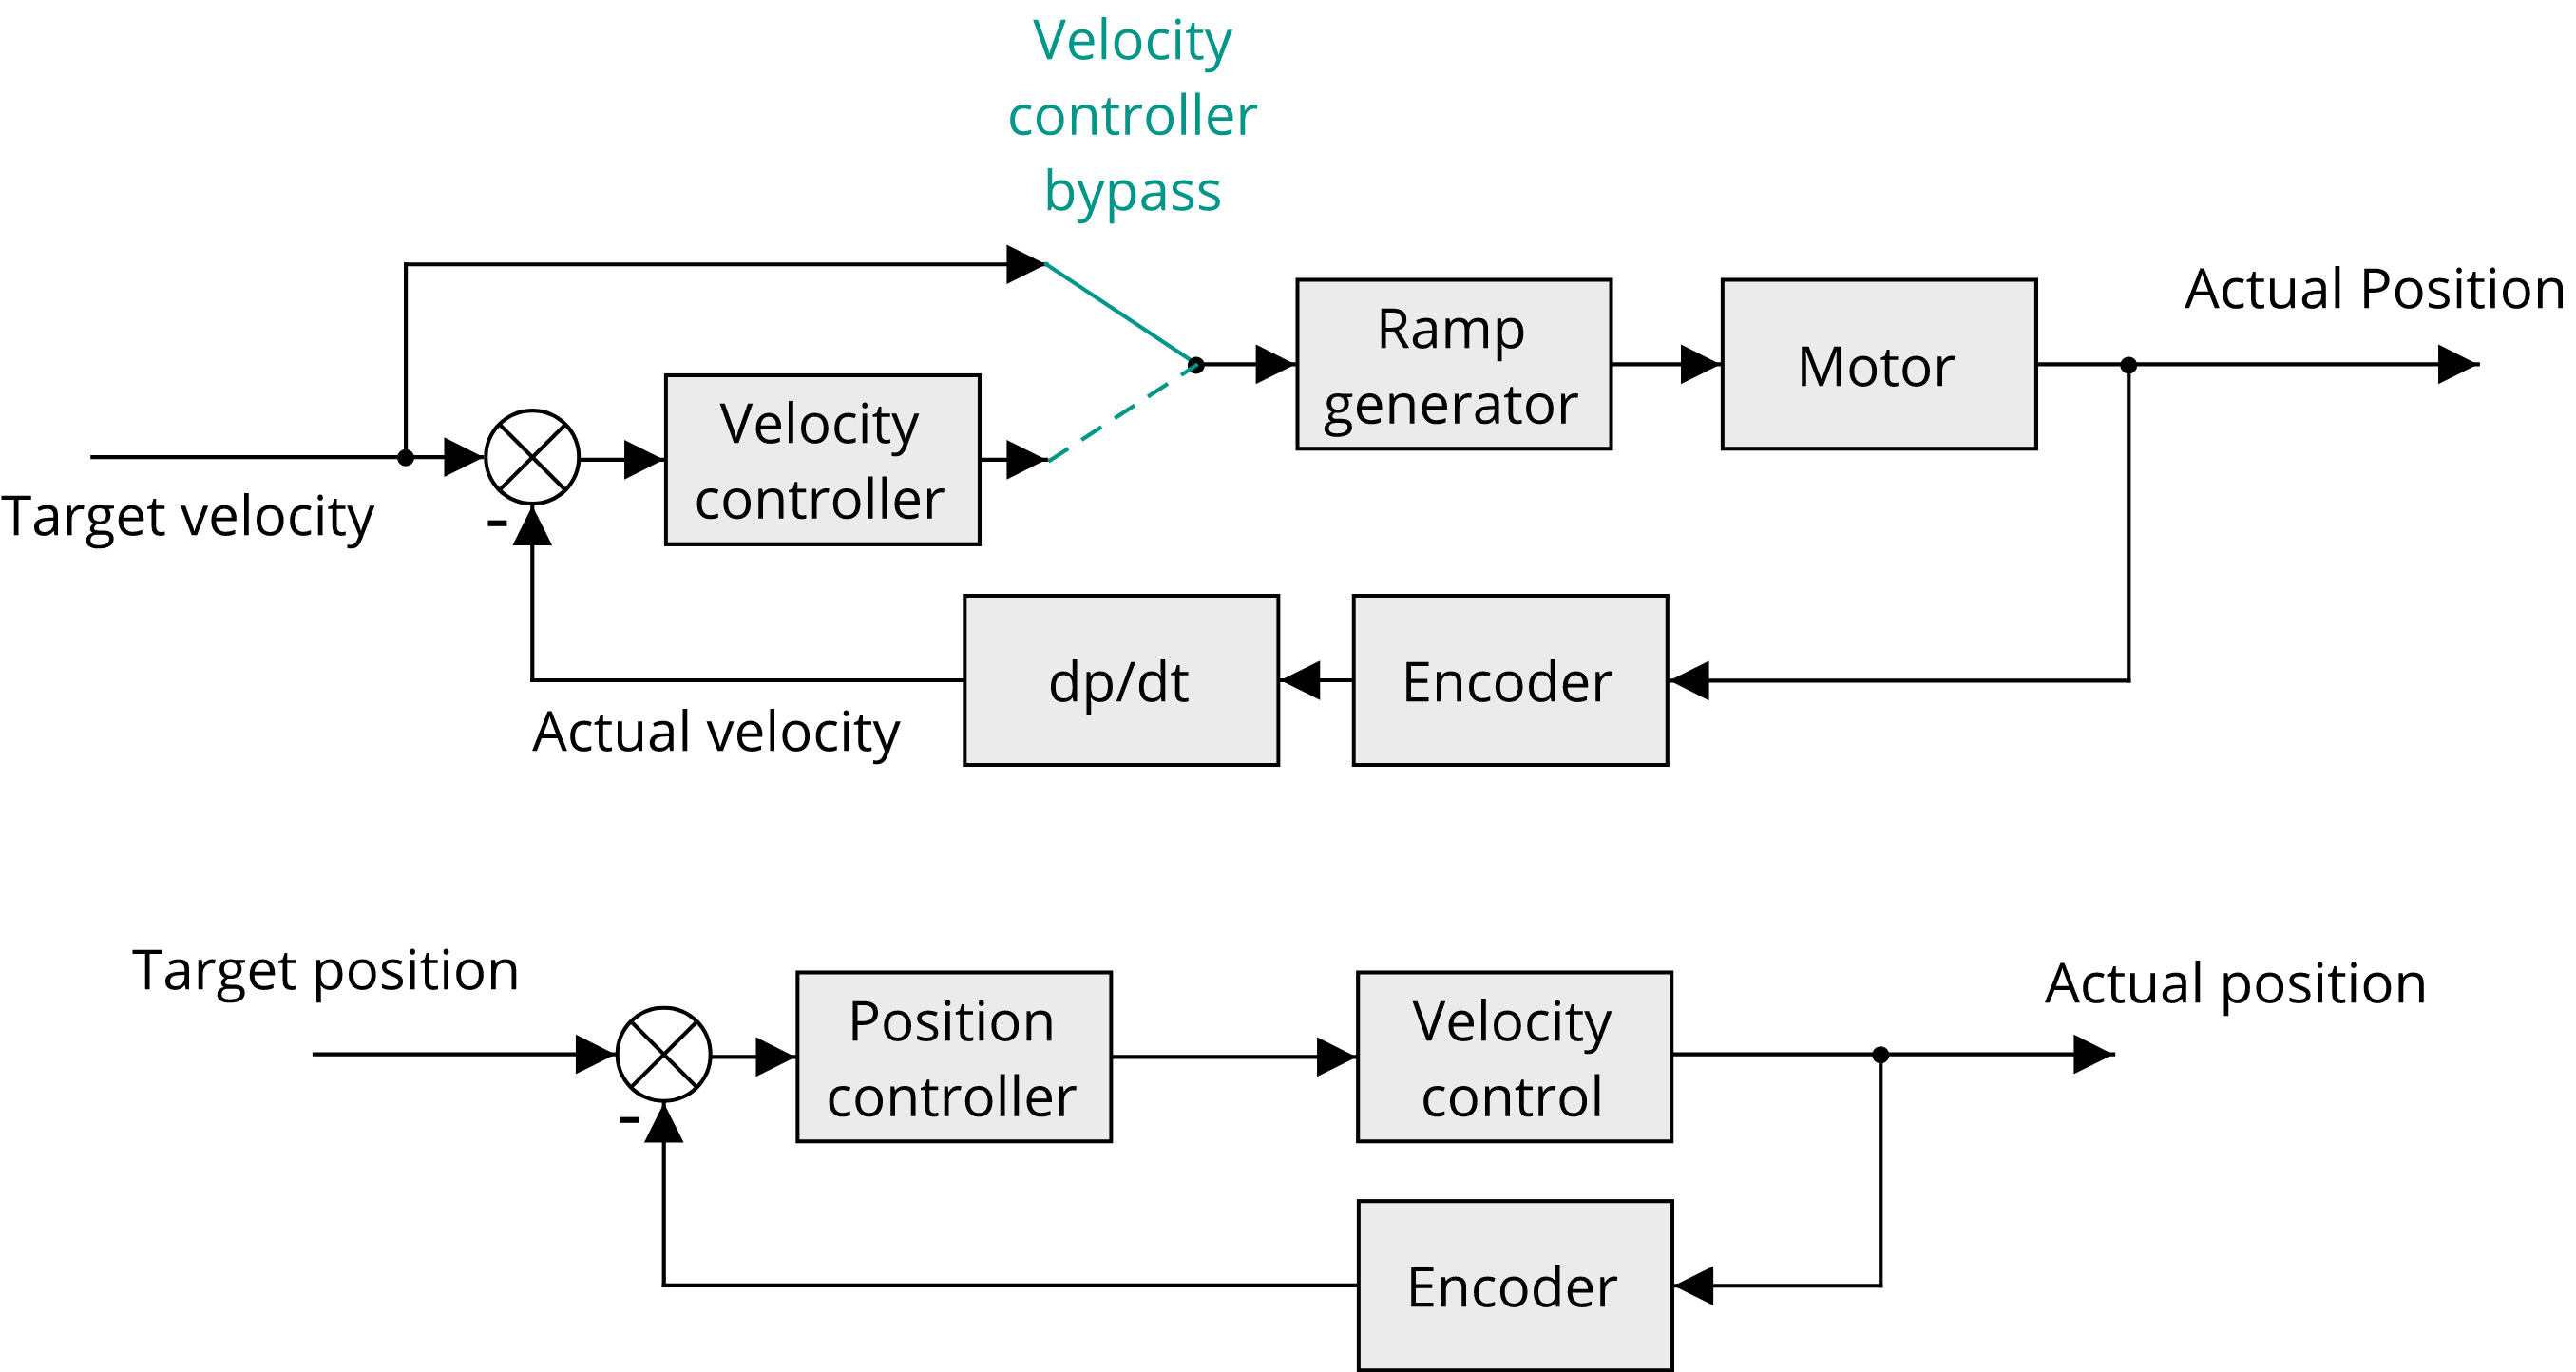
\includegraphics[width=\textwidth]{obrazky/motion_control}
    \caption{Motion control schematic.}
    \label{fig:motion_control}
\end{figure}
